\section{Topics covered}
\begin{itemize}
\item Architectural design decisions
\item Architectural views
\item Architectural patterns
\item Application architectures
\end{itemize}

\section{Software architecture}
\begin{itemize}
\item The design process for identifying the sub-systems making up a system and the framework for sub-system control and communication is architectural design.
\item The output of this design process is a description of the software architecture.
\end{itemize}

\section{Architectural design}
\begin{itemize}

\item An early stage of the system design process.

\item Represents the link between specification and design processes.

\item Often carried out in parallel with some specification activities.

\item It involves identifying major system components and their communications.

\end{itemize}
\section{The architecture of a packing robot control system}
\begin{figure}[h!]
    \centering
    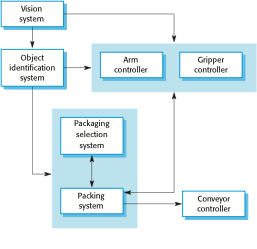
\includegraphics[width = 0.8\textwidth]{./figures/L3_1.png}
    \caption{}
    \label{fig:L3_1}
\end{figure}

\section{Architectural abstraction}
\begin{itemize}

\item Architecture in the small is concerned with the architecture of individual programs. At this level, we are concerned with the way that an individual program is decomposed into components.

\item Architecture in the large is concerned with the architecture of complex enterprise systems that include other systems, programs, and program components. These enterprise systems are distributed over different computers, which may be owned and managed by different companies.


\end{itemize}
\section{Advantages of explicit architecture}
\begin{itemize}
\item Stakeholder communication

 \item Architecture may be used as a focus of discussion by system stakeholders.

\item System analysis

 \item Means that analysis of whether the system can meet its non-functional requirements is possible.

\item Large-scale reuse

 \item The architecture may be reusable across a range of systems  \item Product-line architectures may be developed.
Architectural representations

\item Simple, informal block diagrams showing entities and relationships are the most frequently used method for documenting software architectures.

\item But these have been criticised because they lack semantics, do not show the types of relationships between entities nor the visible properties of entities in the architecture.

\item Depends on the use of architectural models.The requirements for model semantics depends on how the models are used.
Box and line diagrams
\item Very abstract - they do not show the nature of component relationships nor the externally visible properties of the sub-systems.

\item However, useful for communication with stakeholders and for project planning.


\end{itemize}
\section{Use of architectural models}
\begin{itemize}

\item As a way of facilitating discussion about the system design

 \item A high-level architectural view of a system is useful for communication with system stakeholders and project planning because it is not cluttered with detail. Stakeholders can relate to it and understand an abstract view of the system. They can then discuss the system as a whole without being confused by detail.

\item As a way of documenting an architecture that has been designed

 \item The aim here is to produce a complete system model that shows the different components in a system, their interfaces and their connections.
\end{itemize}
\section{Architectural design decisions}
\begin{itemize}

\item Architectural design is a creative process so the process differs depending on the type of system being developed.

\item However, a number of common decisions span all design processes and these decisions affect the non-functional characteristics of the system.
\end{itemize}
\section{Architectural design decisions}
\begin{itemize}

\item Is there a generic application architecture that can be used?

\item How will the system be distributed?

\item What architectural styles are appropriate?

\item What approach will be used to structure the system?

\item How will the system be decomposed into modules?

\item What control strategy should be used?

\item How will the architectural design be evaluated?

\item How should the architecture be documented?

\end{itemize}
\section{Architecture reuse}
\begin{itemize}
\item Systems in the same domain often have similar architectures that reflect domain concepts.

\item Application product lines are built around a core architecture with variants that satisfy particular customer requirements.

\item The architecture of a system may be designed around one of more architectural patterns or ‘styles’.

 \item These capture the essence of an architecture and can be instantiated in different ways.
 \item Discussed later in this lecture.

\end{itemize}
\section{Architecture and system characteristics}
\begin{itemize}
\item Performance

 \item Localise critical operations and minimise communications. Use large rather than fine-grain components.

\item Security

 \item Use a layered architecture with critical assets in the inner layers. \item Safety
 \item Localise safety-critical features in a small number of sub-systems. \item Availability
 \item Include redundant components and mechanisms for fault tolerance.

\item Maintainability

 \item Use fine-grain, replaceable components.
\end{itemize}
\section{Architectural views}
\begin{itemize}
\item What views or perspectives are useful when designing and documenting a system’s architecture?

\item What notations should be used for describing architectural models?

\item Each architectural model only shows one view or perspective of the system.

 \item It might show how a system is decomposed into modules, how the run-time processes interact or the different ways in which system components are distributed across a network. For both design and documentation, you usually need to present multiple views of the software architecture.

\end{itemize}
\section{4 + 1 view model of software architecture}
\begin{itemize}
\item A logical view, which shows the key abstractions in the system as objects or object classes.

\item A process view, which shows how, at run-time, the system is composed of interacting processes.

\item A development view, which shows how the software is decomposed for development.

\item A physical view, which shows the system hardware and how software components are distributed across the processors in the system.

\item Related using use cases or scenarios (+1)
\end{itemize}
\section{Architectural patterns}
\begin{itemize}
\item Patterns are a means of representing, sharing and reusing knowledge.

\item An architectural pattern is a stylized description of good design practice, which has been tried and tested in different environments.

\item Patterns should include information about when they are and when the are not useful.

\item Patterns may be represented using tabular and graphical descriptions.

\end{itemize}
\section{The Model-View-Controller (MVC) pattern}

\begin{table}[h!]
\centering
\begin{tabular}{ |p{3cm}|p{8cm}|  }
\hline
Name & MVC (Model-View-Controller) \\
\hline
\hline
Description & Separates presentation and interaction from the system data. The system is structured into three logical components that interact with each other. The Model component manages the system data and associated operations on that data. The View component defines and manages how the data is presented to the user. The Controller component manages user interaction (e.g., key presses, mouse clicks, etc.) and passes these interactions to the View and the Model. See Figure 6.3.\\
\hline
Example & Figure 6.4 shows the architecture of a web-based application system organized using the MVC pattern.\\
\hline
When used & Used when there are multiple ways to view and interact with data. Also used when the future requirements for interaction and presentation of data are unknown.\\
\hline
Advantages & Allows the data to change independently of its representation and vice versa. Supports presentation of the same data in different ways with changes made in one representation shown in all of them.\\
\hline
Disadvantages & Can involve additional code and code complexity when the data model and interactions are simple.\\
\hline
\end{tabular}

\label{table:T2_3}
\end{table}
\section{The organization of the Model-View-Controller}
\begin{figure}[h!]
    \centering
    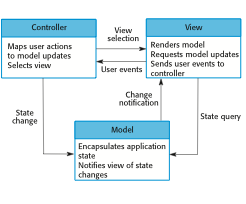
\includegraphics[width = 0.8\textwidth]{./figures/L3_2.png}
    \caption{}
    \label{fig:L3_2}
\end{figure}
\newpage
\section{Web application architecture using the MVC pattern}
\begin{figure}[h!]
    \centering
    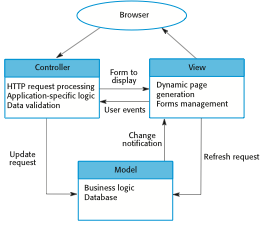
\includegraphics[width = 0.8\textwidth]{./figures/L3_3.png}
    \caption{}
    \label{fig:L3_3}
\end{figure}

\section{Layered architecture}
\begin{itemize}
\item Used to model the interfacing of sub-systems.

\item Organises the system into a set of layers (or abstract machines) each of which provide a set of services.

\item Supports the incremental development of sub-systems in different layers. When a layer interface changes, only the adjacent layer is affected.

\item However, often artificial to structure systems in this way.

\end{itemize}
\newpage
\section{The Layered architecture pattern}


\begin{table}[h!]
\centering
\begin{tabular}{ |p{3cm}|p{8cm}|  }
\hline
Name & Layered architecture\\
\hline
\hline
Description & Organizes the system into layers with related functionality associated with each layer. A layer provides services to the layer above it so the lowest-level layers represent core services that are likely to be used throughout the system. See Figure 6.6.\\
\hline
Example & A layered model of a system for sharing copyright documents held in different libraries, as shown in Figure 6.7.\\
\hline
When used & Used when building new facilities on top of existing systems; when the development is spread across several teams with each team responsibility for a layer of functionality; when there is a requirement for multi-level security.\\
\hline
Advantages & Allows replacement of entire layers so long as the interface is maintained. Redundant facilities (e.g., authentication) can be provided in each layer to increase the dependability of the system.\\
\hline
Disadvantages & In practice, providing a clean separation between layers is often difficult and a high-level layer may have to interact directly with lower-level layers rather than through the layer immediately below it. Performance can be a problem because of multiple levels of interpretation of a service request as it is processed at each layer.\\
\hline
\end{tabular}

\label{table:T2_3}
\end{table}

\newpage
\section{A generic layered architecture}
\begin{figure}[h!]
    \centering
    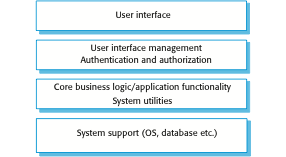
\includegraphics[width = 0.8\textwidth]{./figures/L3_4.png}
    \caption{}
    \label{fig:L3_4}
\end{figure}

\section{The architecture of the LIBSYS system}
\begin{figure}[h!]
    \centering
    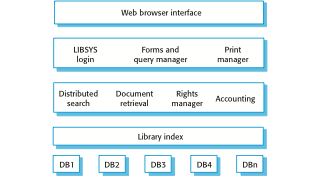
\includegraphics[width = 0.8\textwidth]{./figures/L3_5.png}
    \caption{}
    \label{fig:L3_5}
\end{figure}

\section{Key points}
\begin{itemize}

\item A software architecture is a description of how a software system is organized.

\item Architectural design decisions include decisions on the type of application, the distribution of the system, the architectural styles to be used.

\item Architectures may be documented from several different perspectives or viewssuch as a conceptual view, a logical view, a process view, and a development view.

\item Architectural patterns are a means of reusing knowledge about generic system architectures. They describe the architecture, explain when it may be used and describe its advantages and disadvantages.


\end{itemize}
\section{Repository architecture}
\begin{itemize}
\item Sub-systems must exchange data. This may be done in two ways:

 \item Shared data is held in a central database or repository and may be accessed by all sub-systems;
 \item Each sub-system maintains its own database and passes data explicitly to other sub-systems.

\item When large amounts of data are to be shared, the repository model of sharing is most commonly used a this is an efficient data sharing mechanism.


\end{itemize}
\section{A repository architecture for an IDE}
\begin{figure}[h!]
    \centering
    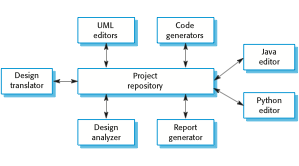
\includegraphics[width = 0.8\textwidth]{./figures/L3_6.png}
    \caption{}
    \label{fig:L3_6}
\end{figure}
\newpage
\section{The Repository pattern}


\begin{table}[h!]
\centering
\begin{tabular}{ |p{3cm}|p{8cm}|  }
\hline
Name & Repository\\
\hline
\hline
Description & All data in a system is managed in a central repository that is accessible to all system components. Components do not interact directly, only through the repository.\\
\hline
Example & Figure 6.9 is an example of an IDE where the components use a repository of system design information. Each software tool generates information which is then available for use by other tools.\\
\hline
When used & You should use this pattern when you have a system in which large volumes of information are generated that has to be stored for a long time. You may also use it in data-driven systems where the inclusion of data in the repository triggers an action or tool.\\
\hline
Advantages & Components can be independent—they do not need to know of the existence of other components. Changes made by one component can be propagated to all components. All data can be managed consistently (e.g., backups done at the same time) as it is all in one place.\\
\hline
Disadvantages & The repository is a single point of failure so problems in the repository affect the whole system. May be inefficiencies in organizing all communication through the repository. Distributing the repository across several computers may be difficult.\\
\hline
\end{tabular}

\label{table:T2_3}
\end{table}



\section{Client-server architecture}
\begin{itemize}

\item Distributed system model which shows how data and processing is distributed across a range of components.

 \item Can be implemented on a single computer.

\item Set of stand-alone servers which provide specific services such as printing, data management, etc.

\item Set of clients which call on these services. \item Network which allows clients to access servers.

\end{itemize}
\section{The Client–server pattern}

\begin{table}[h!]
\centering
\begin{tabular}{ |p{3cm}|p{8cm}|  }
\hline
Name & Client-server\\
\hline
\hline
Description & In a client–server architecture, the functionality of the system is organized into services, with each service delivered from a separate server. Clients are users of these services and access servers to make use of them.\\
\hline
Example & Figure 6.11 is an example of a film and video/DVD library organized as a client–server system.\\
\hline
When used & Used when data in a shared database has to be accessed from a range of locations. Because servers can be replicated, may also be used when the load on a system is variable.\\
\hline
Advantages & The principal advantage of this model is that servers can be distributed across a network. General functionality (e.g., a printing service) can be available to all clients and does not need to be implemented by all services.\\
\hline
Disadvantages & Each service is a single point of failure so susceptible to denial of service attacks or server failure. Performance may be unpredictable because it depends on the network as well as the system. May be management problems if servers are owned by different organizations.\\
\hline
\end{tabular}

\label{table:T2_3}
\end{table}
\newpage
\section{A client–server architecture for a film library}
\begin{figure}[h!]
    \centering
    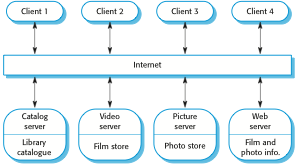
\includegraphics[width = 0.8\textwidth]{./figures/L3_7.png}
    \caption{}
    \label{fig:L3_7}
\end{figure}

\section{Pipe and filter architecture}
\begin{itemize}
\item Functional transformations process their inputs to produce outputs.

\item May be referred to as a pipe and filter model (as in UNIX shell).

\item Variants of this approach are very common. When transformations are sequential, this is a batch sequential model which is extensively used in data processing systems.

\item Not really suitable for interactive systems.
\end{itemize}

\newpage
\section{The pipe and filter pattern}

\begin{table}[h!]
\centering
\begin{tabular}{ |p{3cm}|p{8cm}|  }
\hline
Name & Pipe and filter\\
\hline
\hline
Description & The processing of the data in a system is organized so that each processing component (filter) is discrete and carries out one type of data transformation. The data flows (as in a pipe) from one component to another for processing.\\
\hline
Example & Figure 6.13 is an example of a pipe and filter system used for processing invoices.\\
\hline
When used & Commonly used in data processing applications (both batch- and transaction-based) where inputs are processed in separate stages to generate related outputs.\\
\hline
Advantages & Easy to understand and supports transformation reuse. Workflow style matches the structure of many business processes. Evolution by adding transformations is straightforward. Can be implemented as either a sequential or concurrent system.\\
\hline
Disadvantages & The format for data transfer has to be agreed upon between communicating transformations. Each transformation must parse its input and unparse its output to the agreed form. This increases system overhead and may mean that it is impossible to reuse functional transformations that use incompatible data structures.\\
\hline
\end{tabular}

\label{table:T2_3}
\end{table}

\newpage
\section{An example of the pipe and filter architecture}
\begin{figure}[h!]
    \centering
    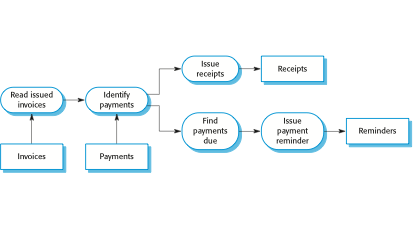
\includegraphics[width = 0.8\textwidth]{./figures/L3_8.png}
    \caption{}
    \label{fig:L3_8}
\end{figure}

\section{Application architectures}
\begin{itemize}
\item Application systems are designed to meet an organisational need.

\item As businesses have much in common, their application systems also tend to have a common architecture that reflects the application requirements.

\item A generic application architecture is an architecture for a type of software system that may be configured and adapted to create a system that meets specific requirements.

\end{itemize}
\section{Use of application architectures}
\begin{itemize}
\item As a starting point for architectural design. \item As a design checklist.
\item As a way of organising the work of the development team. \item As a means of assessing components for reuse.
\item As a vocabulary for talking about application types.

\end{itemize}
\section{Examples of application types}
\begin{itemize}
\item Data processing applications

 \item Data driven applications that process data in batches without explicit user intervention during the processing.

\item Transaction processing applications

 \item Data-centred applications that process user requests and update information in a system database.

\item Event processing systems

 \item Applications where system actions depend on interpreting events from the system’s environment.

\item Language processing systems

 \item Applications where the users’ intentions are specified in a formal language that is processed and interpreted by the system.
\end{itemize}
\section{Application type examples}
\begin{itemize}
\item Focus here is on transaction processing and language processing systems.

\item Transaction processing systems  \item E-commerce systems;  \item Reservation systems.
\item Language processing systems  \item Compilers;
 \item Command interpreters.


\end{itemize}
\section{Transaction processing systems}
\begin{itemize}
\item Process user requests for information from a database or requests to update the database.

\item From a user perspective a transaction is:

 \item Any coherent sequence of operations that satisfies a goal;  \item For example - find the times of flights from London to Paris.
\item Users make asynchronous requests for service which are then processed by a transaction manager.


\end{itemize}
\section{The structure of transaction processing applications}
\begin{figure}[h!]
    \centering
    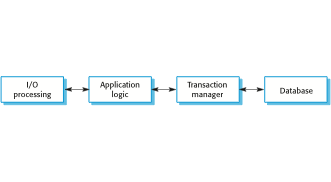
\includegraphics[width = 0.8\textwidth]{./figures/L3_9.png}
    \caption{}
    \label{fig:L3_9}
\end{figure}




\section{The software architecture of an ATM system}
\begin{figure}[h!]
    \centering
    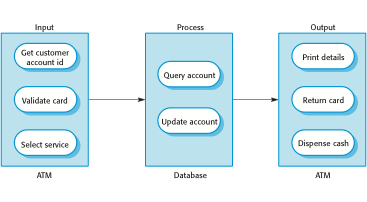
\includegraphics[width = 0.8\textwidth]{./figures/L3_10.png}
    \caption{}
    \label{fig:L3_10}
\end{figure}


\section{Information systems architecture}
\begin{itemize}
\item Information systems have a generic architecture that can be organised as a layered architecture.

\item These are transaction-based systems as interaction with these systems generally involves database transactions.

\item Layers include:  \item The user interface  \item User communications  \item Information retrieval  \item System database

\end{itemize}
\section{Layered information system architecture}
\begin{figure}[h!]
    \centering
    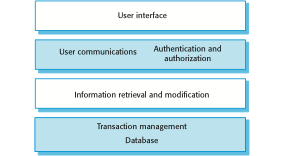
\includegraphics[width = 0.8\textwidth]{./figures/L3_11.png}
    \caption{}
    \label{fig:L3_11}
\end{figure}

\newpage
\section{The architecture of the MHC-PMS}
\begin{figure}[h!]
    \centering
    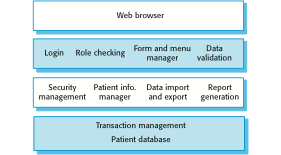
\includegraphics[width = 0.8\textwidth]{./figures/L3_12.png}
    \caption{}
    \label{fig:L3_12}
\end{figure}

\section{Web-based information systems}
\begin{itemize}
\item Information and resource management systems are now usually web-based systems where the user interfaces are implemented using a web browser.

\item For example, e-commerce systems are Internet-based resource management systems that accept electronic orders for goods or services and then arrange delivery of these goods or services to the customer.

\item In an e-commerce system, the application-specific layer includes additional functionality supporting a ‘shopping cart’ in which users can place a number of items in separate transactions, then pay for them all together in a single transaction.

\end{itemize}
\section{Server implementation}
\begin{itemize}
\item These systems are often implemented as multi-tier client server/architectures (discussed in Chapter 18)

 \item The web server is responsible for all user communications, with the user interface implemented using a web browser;
 \item The application server is responsible for implementing application-specific logic as well as information storage and retrieval requests;
 \item The database server moves information to and from the database and handles transaction management.


\end{itemize}
\section{Language processing systems}
\begin{itemize}
\item Accept a natural or artificial language as input and generate some other representation of that language.

\item May include an interpreter to act on the instructions in the language that is being processed.

\item Used in situations where the easiest way to solve a problem is to describe an algorithm or describe the system data

 \item Meta-case tools process tool descriptions, method rules, etc and generate tools.


\end{itemize}
\section{The architecture of a language processing system}
\begin{figure}[h!]
    \centering
    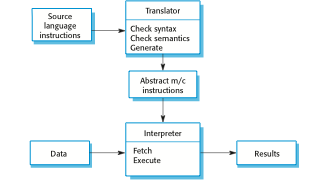
\includegraphics[width = 0.8\textwidth]{./figures/L3_13.png}
    \caption{}
    \label{fig:L3_13}
\end{figure}




\section{Compiler components}
\begin{itemize}
\item A lexical analyzer, which takes input language tokens and converts them to an internal form.

\item A symbol table, which holds information about the names of entities (variables, class names, object names, etc.) used in the text that is being translated.

\item A syntax analyzer, which checks the syntax of the language being translated.

\item A syntax tree, which is an internal structure representing the program being compiled.

Compiler components

\item A semantic analyzer that uses information from the syntax tree and the symbol table to check the semantic correctness of the input language text.

\item A code generator that ‘walks’ the syntax tree and generates abstract machine code.

\end{itemize}
\section{A pipe and filter compiler architecture}
\begin{figure}[h!]
    \centering
    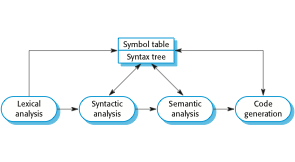
\includegraphics[width = 0.8\textwidth]{./figures/L3_14.png}
    \caption{}
    \label{fig:L3_14}
\end{figure}

\newpage
\section{A repository architecture for a language processing system}
\begin{figure}[h!]
    \centering
    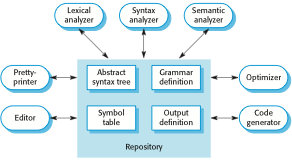
\includegraphics[width = 0.8\textwidth]{./figures/L3_15.png}
    \caption{}
    \label{fig:L3_15}
\end{figure}


\section{Key points}
\begin{itemize}
\item Models of application systems architectures help us understand and compare applications, validate application system designs and assess large-scale components for reuse.

\item Transaction processing systems are interactive systems that allow information in a database to be remotely accessed and modified by a number of users.

\item Language processing systems are used to translate texts from one language into another and to carry out the instructions specified in the input language. They include a translator and an abstract machine that executes the generated language.
\end{itemize}
